%----------------------------------------------------------------------------------------
% PACKAGES AND OTHER DOCUMENT CONFIGURATIONS
%----------------------------------------------------------------------------------------

\documentclass[12pt]{article}
\usepackage[english]{babel}
\usepackage[utf8x]{inputenc}
\usepackage{amsmath}
\usepackage{graphicx}
\usepackage[colorinlistoftodos]{todonotes}

\begin{document}

\begin{titlepage}

\newcommand{\HRule}{\rule{\linewidth}{0.5mm}} % Defines a new command for the horizontal lines, change thickness here

\center % Center everything on the page

%----------------------------------------------------------------------------------------
% LOGO SECTION
%----------------------------------------------------------------------------------------

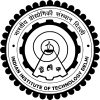
\includegraphics{logo.png}\\[1cm] % Include a department/university logo - this will require the graphicx package
 
 
%----------------------------------------------------------------------------------------
% HEADING SECTIONS
%----------------------------------------------------------------------------------------

\textsc{\LARGE Indian Institute of Technology, Delhi}\\[1.5cm] % Name of your university/college
\textsc{\Large B.Tech Project Report}\\[0.5cm] % Major heading such as course name
% \textsc{\large B.Tech Project}\\[0.5cm] % Minor heading such as course title

%----------------------------------------------------------------------------------------
% TITLE SECTION
%----------------------------------------------------------------------------------------

\HRule \\[0.4cm]
{ \huge \bfseries Utility Package for Vision Lab}\\[0.4cm] % Title of your document
\HRule \\[1.5cm]
 
%----------------------------------------------------------------------------------------
% AUTHOR SECTION
%----------------------------------------------------------------------------------------

\begin{minipage}{0.4\textwidth}
\begin{flushleft} \large
\emph{Author:}\\
Aman \textsc{Bhatia} % Your name
\end{flushleft}
\end{minipage}
~
\begin{minipage}{0.4\textwidth}
\begin{flushright} \large
\emph{Supervisor:} \\
Prof. Subhashis \textsc{Banerjee} % Supervisor's Name
\end{flushright}
\end{minipage}\\[2cm]

% If you don't want a supervisor, uncomment the two lines below and remove the section above
%\Large \emph{Author:}\\
%John \textsc{Smith}\\[3cm] % Your name

%----------------------------------------------------------------------------------------
% DATE SECTION
%----------------------------------------------------------------------------------------

{\large November 18, 2016}\\[2cm] % Date, change the \today to a set date if you want to be precise


%----------------------------------------------------------------------------------------

\vfill % Fill the rest of the page with whitespace

\end{titlepage}


\section{Introduction}

We will discuss various features of the package as well as a brief introduction of the various techniques used. The package supports various key tasks that are very frequently needed while working with images. The project includes various non-rudimentary techniques for the task of Image Segmentation, Background Subtraction, Motion Segmentation, Image Resizing and Object Removal by Seam Carving and Photomontaging.

In the next section, we will discuss each of these techniques in detail along with proper instruction of how to use them in the package.\\

\section{Package Functions}

\subsection{Image Segmentation}

Image Segmentation is the process of segmenting an image into parts such that each part represent a constituent. Constituent can be anything like an object, a similar color region etc. There are various common techniques for image segmentation such as K-means clustering, Histogram Based Segmentation etc. However, this package implements various non-rudimentary techniques, implementations of some of which are hard to find.\\

\subsubsection{Mean-Shift Image Segmentation}

It is an iterative algorithm. Each pixel is associated with a feature vector. A feature vector can be anything like (x,y,r,g,b) or just (r,g,b), or (h,s,v) etc. Then for each pixel, mean is calculated over pixel neighbourhood and the pixel is assigned that mean. This is done until convergence.\\

\textbf{Input Parameters:} User have to specify spatial and range radius. Spatial radius signifies larger neighbourhood(for x and y) and range radius signifies larger RGB bandwidth. Larger the spatial radius, more time it will take to segment.\\

\subsubsection{Efficient Graph-Based Image Segmentation(Local Variance)}

Here, we form a graph corresponding to the image to segment. Graph is formed with nodes representing pixels \& edges representing pixel neighbourhood. Edge weights determine similarity between two pixels. Similarity criteria can be Euclidean Distance between feature vectors. Connected Components are found in the graph using modified Kruskal Algorithm which takes into account local variation of a connected component.\\

\textbf{Usage:} The user has three track-bars(sliders) to play with. First is the Gaussian blur sigma of the Gaussian kernel that is used to blur the image in the beginning. Second is parameter `k' of the modified Kruskal Algo. It controls the local variance of the cluster. Larger the k, bigger the cluster size. Third is minimum component size which controls the minimum allowed size of the clusters in the graph.\\

\subsubsection{Normalized Cut Image Segmentation}

N-cut : Suppose the cut divides the graph in two clusters A and B.

$$ w(A,B) = sum\  of\  all\  edge\  weights\  from\  cluster\  A\  to\  B $$
$$ Ncut(A,B) = w(A,B)\bigg( \frac{1}{w(A,V)} + \frac{1}{w(B,V)} \bigg) $$

 We are trying to find out a minimum energy cut in the graph. The problem with min-cut is that it many times separate just a single node of the graph. N-cut takes into account the size of the components that are getting formed and hence, gives far better results then min-cut.\\
 
 Here also, a graph is formed with nodes representing pixels \& edges representing pixel neighbourhood. Edge weights determine similarity between two pixels. Normalized cut is then found in this graph recursively.\\
 
 The image needs to be super-pixel first because the complexity of normalized cut is high. By default, for any image 400 super pixels are found first and then N-cut is applied.\\



\subsubsection{Graph Cuts}

Suppose we have a cut in the graph which cuts the graph in two labels ($\alpha$ and $\beta$). $\alpha$ -swap is when several pixels with label $\alpha$ are changed to label $\beta$, and those with label $\beta$ are changed to label $\alpha$. $\alpha$-expansion is when several pixels with label $\beta$ are changed to label $\alpha$ but not the other way. These two trigger wide change in energy of the graph and thus converges in very few iterations.\\

So, a graph is formed in the same way as in above techniques and any cut is found in the graph. Then $\alpha$-$\beta$ swap and $\alpha$-expansion are applied. This algorithm is very fast(almost real time) and by far, gives the best results.\\

\textbf{Input Parameters:} User needs to give the number of clusters to segment the image. Once the image is segmented, user can control the granularity of segments by pressing `i' and decreasing it by pressing `d', in real-time.\\


\subsection{Seam Carving}

Seam Carving is an algorithm for content aware image resizing. When we try to resize an image, the whole image gets shrunken or elongated. Seam Carving tries to keep the relevant information, on the basis of the content in the image and only removes(adds) the part which contains less information. This gives far better results as compared to normal image resizing.\\

\subsubsection{Image Resizing}
 A seam is a continuous path from top to bottom(or left to right) of the image. Various minimum energy seams(seams of least importance) are calculated and removed(added) from the image. \\

\textbf{Input Parameters:} User has to input number of rows(or columns) to delete and insert in the image. Then it will find the required seams in the image and remove it in real time. Seams are shown in red and user can see which seams are getting removed from the image.\\


\subsubsection{Object Removal and Saving}
Another application of Seam Carving is Object removal or Saving from the image. A user can draw over an object to remove(or save) it from the image. When user draws over an object to remove it, the energy of those pixels is set to $-\infty$ and so all the seams now pass through those pixels, getting the object removed.\\

\subsection{Photo-montage}
Photo-montage is the process of making a composite photograph by cutting, gluing, rearranging and overlapping two or more photographs into a new image. I have incorporated the binary provided on the web-page of the research paper. Link to the paper can be found in the reference section.\\

\textbf{Usage Instructions:} Go to File and select New Composite. Then in the Composite, go to File and select Load Stack. Here, select all the images from which you want to form the composite. Then in each image of the stack, draw over the part you want to copy to final composite from this image.

\subsection{Background Subtraction}

Background subtraction, also known as Foreground Detection, is a technique in the fields of image processing and computer vision wherein an image's foreground is extracted for further processing (object recognition etc.).\\

\textbf{Usage Instructions:} For the task of Background Subtraction, I have used createBackgroundSubtractorMOG2() function implemented in opencv. User just need to select a video, and the function would output the foreground mask based on consecutive frames of the video.\\


\subsection{Motion Segmentation}

Motion Segmentation is the process of separating regions, features, or trajectories from a video sequence on basis of their motion. I used optical flow followed by k-means clustering to recognize different motions in the scene. Firstly, optical flow is calculated between consecutive frames of the video using `calcOpticalFlowFarneback` method of Opencv. This returns motion in x and y direction, so we calculated magnitude and direction of motion at each pixel. Then I used k-means clustering where user have to give as input the no. of clusters(default no. of clusters = 2).\\

I tested several videos with 3-4 objects in different motion and this method successfully segmented the motion. For real time usage, the video sequence is downsampled and the motion is detected on the downsampled video. Then we upscale the determined motion to the actual size.\\


\section{Future Work}

The implementation of Seam Carving does not contain support for removal of seams of minimum energy in optimal order, i.e., when both horizontal and vertical seams are to be removed, the program will first remove all the vertical seams and then remove all the horizontal seams. Efficient dynamic programming based algorithms exist for calculating optimal order of removal of seams. Those algorithms can be incorporated in the existing implementation.\\

I have implemented optical-flow based motion segmentation. However, various other algorithms based on Layers, Statistic theory, Graph-Cuts also exist which can be incorporated in the project.\\

\section{References}

\begin{itemize}
    \item AGARWALA, A., DONTCHEVA, M., AGRAWALA, M., DRUCKER, S., COLBURN, A., CURLESS, B., SALESIN, D., AND COHEN, M. 2004. Interactive digital photomontage. ACM Trans. Graph. 23, 3, 294–302
    
    \item BOYKOV, Y., AND JOLLY, M.-P. 2001. Interactive graph cuts for optimal boundary \& region segmentation of objects in n-d images. In International Conference on Computer Vision, (ICCV), vol. I, 105–112.
    
    \item C. M. CHRISTOUDIAS, B. GEORGESCU, AND P. MEER. Synergism in low level vision. In International Conference on Pattern Recognition., Quebec City, Canada, volume IV, pages 150–155, 2002.
    
    \item D. COMANICIU AND P. MEER. Mean shift: A robust approach toward feature space analysis. IEEE Trans. PAMI, 24:603–619, 2002.
    
    \item J. SHI, C. FOWLKES, D. MARTIN, AND E. SHARON. Graph based image segmentation tutorial. IEEE CVPR 2004.
    
    \item J. SHI AND J. MALIK. Normalized cuts and image segmentation. IEEE Trans. PAMI, 22(8):888–905, 2000.
    
    \item P.F. FELZENSZWALB AND D.P. HUTTENLOCHER. Efficient graph-based image segmentation. IJCV, 59(2):167–181, 2004.
    
    \item S. AVIDAN AND A. SHAMIR. Seam carving for content-aware image resizing. In
SIGGRAPH, 2007.
    

\end{itemize}

% Commands to include a figure:
% \begin{figure}
% \centering
% \includegraphics[width=0.5\textwidth]{frog.jpg}
% \caption{\label{fig:frog}This is a figure caption.}
% \end{figure}


\end{document}